% Copyright (c) 2018 Victorien Elvinger
% Code licensed under GPLv3 (https://www.gnu.org/licenses/gpl-3.0.en.html).
% Content licensed under CC-BY 4.0 (https://creativecommons.org/licenses/by/4.0/).

\documentclass[xcolor=table]{beamer}

% https://tex.stackexchange.com/questions/275600/beamer-themes-on-custom-folder
\makeatletter
  \def\beamer@calltheme#1#2#3{%
    \def\beamer@themelist{#2}
    \@for\beamer@themename:=\beamer@themelist\do
    {\usepackage[{#1}]{\beamer@themelocation/#3\beamer@themename}}}

  \def\themefolder#1{
    \def\beamer@themelocation{#1}
  }
  \def\beamer@themelocation{}

\themefolder{theme}
\usetheme[sectionpage=simple,numbering=fraction]{metropolis}

\usepackage[utf8]{inputenc}
\usepackage{amsmath}
\usepackage{hyperref}
\usepackage{acronym} % \ac[p], \acl[p], \acs[p], \acf[p]

\usepackage[scale=1.5]{ccicons}

\usepackage{listings}
\lstset{
  basicstyle=\footnotesize, 
}

\usepackage{color}
\usepackage{tikz}
\usetikzlibrary{arrows,arrows.meta,calc,positioning,shapes}

\usepackage{transparent}

\graphicspath{{./fig/}}

\usepackage{silence}
\WarningFilter{biblatex}{Patching footnotes failed}
    % Filter warning of biblatex package: "Patching footnotes failed"

\usepackage{appendixnumberbeamer}

% Refs and Footnotes
% ------------------
\usepackage[backend=biber,defernumbers=true,style=trad-plain,sorting=none,maxbibnames=1,maxcitenames=3]{biblatex}
\AtBeginBibliography{\footnotesize}
\setbeamertemplate{bibliography item}[text] % use ref number in bibliography

\renewcommand{\thefootnote}{[\arabic{footnote}]}
    % Footnote style: [footnote-counter]

\newcommand\singlefootnote[1]{%
    % Use this footnote variant when a single footnote is on the page
    % Footnote style: *
    \begingroup
    %\renewcommand\thefootnote{}\footnote{#1}%
    \renewcommand{\thefootnote}{*}\footnote{#1}%
    \addtocounter{footnote}{-1}%
    \endgroup
}

% Colors
% ------
% Prefix every color with 'uc' (user-defined color)

\definecolor{uctrusted}{HTML}{00CC00}

% Subcaption
% ----------
\makeatletter
\let\MYcaption\@makecaption
\makeatother

\usepackage[font=footnotesize]{subcaption}

\makeatletter
\let\@makecaption\MYcaption
\makeatother

\captionsetup{subrefformat=parens}


% Meta-data
% ---------

\author{Victorien Elvinger}
\title{Software Engineering - Architecture and design patterns for Graphical User Interfaces}
\institute{%
    \includegraphics[height=1.6em]{/logo/loria.pdf}\hspace{1.6em}%
    \includegraphics[height=1.6em]{/logo/ul.pdf}\hspace{1.6em}%
    \includegraphics[height=1.6em]{/logo/cnrs.pdf}\hspace{1.6em}%
    \includegraphics[height=1.6em]{/logo/inria.pdf}\hspace{1.6em}%
}
\date{November 2019}

% Content
% -------

\begin{document}

\maketitle

\section{Notions de couplage}

\begin{frame}{Modules}
\begin{itemize}
    \item Un programme est découpé en modules
        \begin{itemize}
            \item Fonctions
            \item Classes et Interfaces
            \item Paquets
        \end{itemize}
\end{itemize}
\end{frame}

\begin{frame}{Dépendances entre modules}
\begin{figure}
    \centering
    \includegraphics<1>[scale=0.7]{fig/cartesian-point.pdf}
    \includegraphics<2>[scale=0.7]{fig/dependency-example.pdf}
\end{figure}
\begin{itemize}
    \item Un module peut dépendre sur un autre
    \begin{itemize}
        \item Une fonction qui appelle une autre fonction
        \item une classe qui hérite d'une autre classe
        \item Une classe en relation cliente avec une autre classe
    \end{itemize}
\end{itemize}
\end{frame}

\begin{frame}{Couplage}
\begin{figure}
    \centering
    \includegraphics<1>[scale=0.7]{fig/cartesian-point.pdf}
    \includegraphics<2>[scale=0.7]{fig/polar-point.pdf}
    \includegraphics<3>[scale=0.7]{fig/diago-rectangle.pdf}
\end{figure}
\begin{itemize}
    \item Degré de dépendance entre deux modules
    \item Difficulté de modifier indépendemment 2 modules fortement couplés
\end{itemize}
\end{frame}

\begin{frame}{Découplage et couplage faible}
\begin{figure}
    \centering
    \begin{subfigure}{0.48\linewidth}
        \centering
        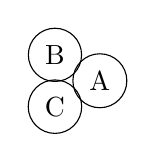
\begin{tikzpicture}
            \node[draw,circle] at (0:0.38) {A};
            \node[draw,circle] at (120:0.38) {B};
            \node[draw,circle] at (240:0.38) {C};
        \end{tikzpicture}
        \caption*{Couplage fort}
    \end{subfigure}
    \begin{subfigure}{0.48\linewidth}
        \centering
        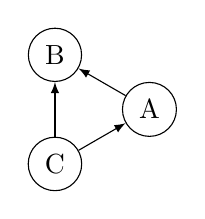
\begin{tikzpicture}
            \node[draw,circle] (A) at (0:0.8) {A};
            \node[draw,circle] (B) at (120:0.8) {B};
            \node[draw,circle] (C) at (240:0.8) {C};
            \draw[<->,-latex] (A) to (B);
            \draw[<->,-latex] (C) to (A);
            \draw[<->,-latex] (C) to (B);
        \end{tikzpicture}
        \caption*{Couplage plus faible}
    \end{subfigure}
\end{figure}
\begin{itemize}
    \item Faciliter la modification et l'ajout de fonctionnalités
    \item Faciliter la réutilisation de modules
    \item Faciliter le travail en équipe
    \item Faciliter l'écriture de tests unitaires
    \item Souvent synonyme d'une bonne conception
\end{itemize}
\end{frame}

% https://www.planttext.com/?text=TP512y8m38Nl-HLbHs53hnv4S20U10-2vsmBhf2radOW_dhNhPiwzVQIx_KbeLldKNpRC83Ndadj69qZfz91gLpZLR01WBAlTpKAbfuarXVzGAaKtJsPwWT64Mtb1u-6CuNmGPyOIuewRysLh9aUlhE3cVSZE5hZNhFFOfaduoVRsuAr-O8GefDbbgqIbQORbIoIViErIalMPBo3KFRzaKyd1TEe7S1umImkZkhCsjHOQ8yXzO_vFPlkDxRIHyEssxhxj2S0

\begin{frame}{Découplage et couplage faible}
\begin{figure}
    \centering
    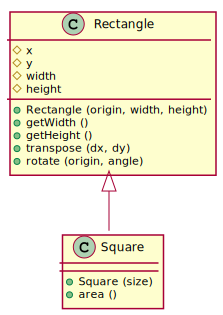
\includegraphics[scale=0.6]{fig/srp.pdf}
\end{figure}
\begin{itemize}
    \item Encapsulation
    \item Préférer la composition à l'héritage
    \item Séparation de préoccupations
    \begin{itemize}
        \item Principe de responsabilité unique
    \end{itemize}
\end{itemize}
\end{frame}

\begin{frame}{Exemple}
\begin{figure}
    \centering
    \includegraphics[scale=0.6]{fig/game.pdf}
\end{figure}
\end{frame}

\section{Design Patterns for Graphical User Interfaces}

\begin{frame}{Arbre de vues}
\begin{figure}
\begin{subfigure}{0.48\linewidth}
    \centering
    \includegraphics<1>[scale=0.32]{fig/ui-example.jpeg}
    \includegraphics<2>[scale=0.32]{fig/ui-view-tree-example.jpeg}
\end{subfigure}
\begin{subfigure}{0.48\linewidth}
    \centering
    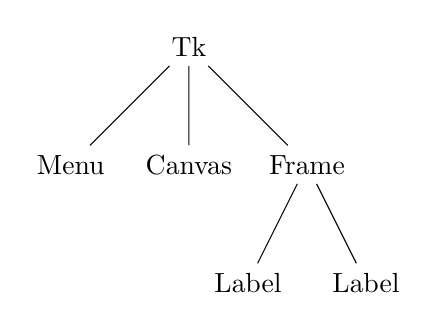
\begin{tikzpicture}
        \node<2> {Tk}
            child {node {Menu}}
            child {node {Canvas}}
            child {node {Frame}
                child {node {Label}}
                child {node {Label}}
            }
        ;
    \end{tikzpicture}
\end{subfigure}
\end{figure}
\begin{itemize}
    \item Une interface est structurée comme un arbre de \emph{vues}
    \item Une \emph{vue} est un élément qui occupe une région de l'écran
\end{itemize}
% Montrer sur une page Web avec l'inspecteur
\end{frame}

\begin{frame}[fragile]{Arbre de vues - Construction procédurale}
\begin{lstlisting}[language=Python]
from tkinter import *
root = Tk()
menu = Menu(root)
canvas = Canvas(root)
bar = Frame(root)
name_info = Label(bar, text="filename:")
size_info = Label(bar, text="size:")
\end{lstlisting}

\begin{itemize}
    \item Construction étape par étape de l'arbre de vues
    \item Utilisation d'un langage de programmation polyvalent
\end{itemize}
\end{frame}

\begin{frame}[fragile]{Arbre de vues - Construction déclarative}
\begin{lstlisting}[language=XML]
<Tk>
    <Menu> ... </Menu>
    <Canvas/>
    <Frame>
        <Label side="left" text="filename:"/>
        <Label side="left" text="size:"/>
    </Frame>
</Tk>
\end{lstlisting}
\begin{itemize}
    \item Représentation directe de l'arbre de vues
    \item Utilisation d'un langage adapté à la représentation d'arbres
\end{itemize}
\end{frame}

\begin{frame}{Avantages de la construction déclarative}
\begin{itemize}
    \item Souvent plus concise
    \item Plus simple pour les non-programmeurs
    \item Développement plus simple d'outils
    \begin{itemize}
        \item Validation de code
        \item Génération d'interface
    \end{itemize}
\end{itemize}
\end{frame}

%\begin{frame}{Interface Graphique}
%\begin{itemize}
%    \item L'interface graphique produit 
%\end{itemize}
%\end{frame}

\begin{frame}{Listener design pattern}
\begin{figure}
    \centering
    \includegraphics[scale=0.75]{fig/observer-pattern.pdf}
\end{figure}
\begin{itemize}
    \item Aussi nommé \emph{Observer design pattern}
    \item Permet à un objet d'avertir ces observateurs que son état a changé en conservant un couplage faible
\end{itemize}
%
% Observable / Publisher / Event source
% Listener / Observer / Subscriber / Event handler
%
\end{frame}

\begin{frame}{Counter example}
\begin{figure}
    \centering
    \includegraphics[scale=0.75]{fig/observable-counter.pdf}
\end{figure}
\end{frame}

\begin{frame}[fragile]{Counter example}
\begin{lstlisting}[language=Java]
public class Counter {
    public void increment () {
        this.value++;
        for (x : this.listeners) { x.changed(this); }
    }
}
public class CounterDisplayer implements CounterListener {
    public void changed(final Counter c) {
        System.out.println(c.getValue());
    }
}
\end{lstlisting}
\end{frame}

\begin{frame}[fragile]{Counter example}
\begin{lstlisting}[language=Java]
public Main {
    public static void main(final String[] args) {
        final Counter c = new Counter();
        final CounterListener v = new CounterDisplayer();
        c.addListener(v)
        
        c.increment(); // 1
        c.increment(); // 2
    }
}
\end{lstlisting}
\end{frame}

\begin{frame}[fragile]{Counter example}
\begin{lstlisting}[language=Java]
public Main {
    public static void main(final String[] args) {
        final Counter c = new Counter();
        final CounterListener v = (c) -> {
            System.out.println(c.getValue());
        }};
        c.addListener(v)
        
        c.increment(); // 1
        c.increment(); // 2
    }
}
\end{lstlisting}
\end{frame}

\begin{frame}{UI conclusion}
\begin{itemize}
    \item Les Entrées / Sorties sont séparées
    \begin{itemize}
        \item La sortie est représentée par un arbre de vues
        \item Les entrées sont traitées par des observateurs attachés à des \emph{vues}
    \end{itemize}
    \item Où se trouve la logique applicative ?
    \begin{itemize}
        \item Les données
        \item Les opérations pour modifier ses données
    \end{itemize}
\end{itemize}
\end{frame}


\section{Architecture MVC}


\begin{frame}{Architecture logicielle}
\begin{itemize}
    \item Manière de découper une application en limitant les couplages
\end{itemize}
\end{frame}

\begin{frame}{Architecture MVC}
\begin{figure}
    \centering
    \begin{subfigure}{0.22\linewidth}
        \centering
        \includegraphics[scale=0.1]{fig/rails.png}
        \caption*{Rails}
    \end{subfigure}
    \begin{subfigure}{0.22\linewidth}
        \centering
        \includegraphics[scale=0.1]{fig/django.png}
        \caption*{Django}
    \end{subfigure}
    \begin{subfigure}{0.22\linewidth}
        \centering
        \includegraphics[scale=0.09]{fig/angular.png}
        \caption*{Angular}
    \end{subfigure}
    \begin{subfigure}{0.22\linewidth}
        \centering
        \includegraphics[scale=0.15]{fig/struts.png}
        \caption*{Struts}
    \end{subfigure}
\end{figure}
\begin{itemize}
    \item Apparition dans les années 80
    \item Séparer la vue de la représentation et la manipulation des données de l'application
    \item Devenue très populaire notamment pour la conception d'applications webs
    \begin{itemize}
        \item Nombreuses variantes de l'architecture
    \end{itemize}
\end{itemize}
\end{frame}

\begin{frame}{Architecture Modèle-Vue-Contrôleur (MVC)}
\begin{figure}
\centering
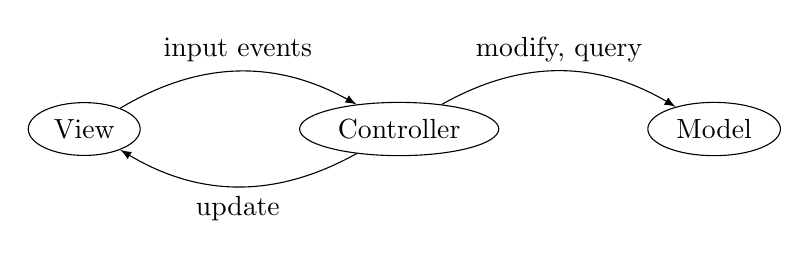
\begin{tikzpicture}[unit/.style={draw,ellipse},link/.style={-latex}]
\node[unit] (V) {View};
\path (V)
    to +(4,0) node[unit] (C) {Controller}
    to +(4*2,0) node[unit] (M) {Model}
    ;
    \path (V) edge[bend left,link] node[above]{input events} (C);
    \path (C) edge[bend left,link] node[below]{update} (V);
    \path (C) edge[bend left,link] node[above]{modify, query} (M);
\end{tikzpicture}
\end{figure}
\begin{description}
    \item[Modèle~:] Représentation des données de l'application, opérations pour modifier et interroger les données
    \item[Vue~:] Interface graphique (Sortie)
    \item[Contrôleur~:] Traitement des entrées des utilisateur·ice·s, modification des données et de la vue
\end{description}
\end{frame}

\begin{frame}{Avantages de MVC}
\begin{figure}
    \centering
    \includegraphics[scale=0.18]{fig/multi-view.png}
\end{figure}
\begin{itemize}
    \item Découplage du modèle de la vue
    \begin{itemize}
        \item Développement en parallèle de la vue et du modèle
        \item Vues multiples pour un même modèle
        \item Réutilisation de la vue pour un autre modèle
    \end{itemize}
\end{itemize}
\end{frame}

\begin{frame}{Architecture MVC}
\begin{figure}
\centering
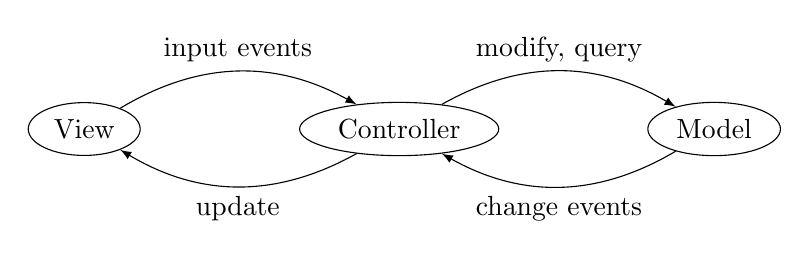
\begin{tikzpicture}[unit/.style={draw,ellipse},link/.style={-latex}]
\node[unit] (V) {View};
\path (V)
    to +(4,0) node[unit] (C) {Controller}
    to +(4*2,0) node[unit] (M) {Model}
    ;
    \path (V) edge[bend left,link] node[above]{input events} (C);
    \path (C) edge[bend left,link] node[below]{update} (V);
    \path (C) edge[bend left,link] node[above]{modify, query} (M);
    \path (M) edge[bend left,link] node[below]{change events} (C);
\end{tikzpicture}
\end{figure}
\begin{itemize}
    \item Le contrôleur doit savoir qu'estc e qui est modifié dans le modèle
    \begin{itemize}
        \item Le contrôleur est couplé assez fortement au modèle
    \end{itemize}
    \item Le modèle est le mieux placé pour savoir ce qui est modifié
\end{itemize}
\end{frame}

\begin{frame}{Architecture MVC}
\begin{figure}
\centering
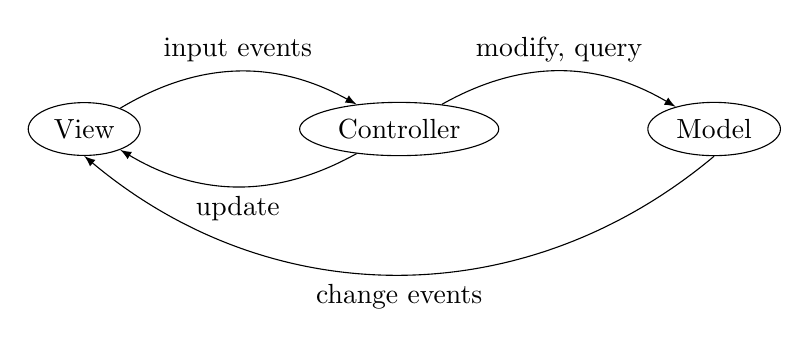
\begin{tikzpicture}[unit/.style={draw,ellipse},link/.style={-latex}]
\node[unit] (V) {View};
\path (V)
    to +(4,0) node[unit] (C) {Controller}
    to +(4*2,0) node[unit] (M) {Model}
    ;
    \path (V) edge[bend left,link] node[above]{input events} (C);
    \path (C) edge[bend left,link] node[below]{update} (V);
    \path (C) edge[bend left,link] node[above]{modify, query} (M);
    \path (M.south) edge[bend left=40,link] node[below]{change events} (V.south);
\end{tikzpicture}
\end{figure}
\begin{itemize}
    \item Le modèle pourrait être modifié par différents contrôleurs
\end{itemize}
\end{frame}



\section{JavaFX}

\end{document}
